\documentclass{article}

\usepackage{graphicx} % Required for the inclusion of images
\usepackage{natbib} % Required to change bibliography style to APA

\setlength\parindent{0pt} % Removes all indentation from paragraphs

 \usepackage{url}

%----------------------------------------------------------------------------------------
%	Report on Argopy Project
%----------------------------------------------------------------------------------------

\title{Report on Argopy Project. \\ CMSC 6950} % Title

\author{Immanuel \textsc{Okpara}} % Author name

\date{\today} % Date for the report

\begin{document}

\maketitle % Insert the title, author and date

% If you wish to include an abstract, uncomment the lines below
% \begin{abstract}
% Abstract text
% \end{abstract}

%----------------------------------------------------------------------------------------
%	SECTION 1
%----------------------------------------------------------------------------------------

\section{Introduction}

Argo is a real-time global ocean in situ observing system.

The ocean is a key component of the Earth climate system. It thus needs a continuous real-time monitoring to help scientists better understand its dynamic and predict its evolution. All around the world, oceanographers have managed to join their efforts and set up a Global Ocean Observing System among which Argo is a key component.\\

Argo is a global network of nearly 4000 autonomous probes measuring pressure, temperature and salinity from the surface to 2000m depth every 10 days. The localisation of these probes is nearly random between the 60th parallels (see live coverage here). All probes data are collected by satellite in real-time, processed by several data centers and finally merged in a single data-set (collecting more than 2 millions of vertical profiles data) made freely available to anyone through a ftp server or monthly zip snapshots.\\

%----------------------------------------------------------------------------------------
%	SECTION 2
%----------------------------------------------------------------------------------------

\section{Installation}
To use Argopy is a python package and is compatible with python versions 3.6, 3.7 and 3.8. 
For this project, the following packages are required;

\begin{enumerate}
\item Argopy
\item Pandas 
\item Matplotlib
\item Numpy 
\end{enumerate}

%----------------------------------------------------------------------------------------
%	SECTION 3
%----------------------------------------------------------------------------------------

\section{Sample Data}

Each Argo probe is an autonomous, free drifting, profiling float, i.e. a probe that can’t control its trajectory but is able to control its buoyancy and thus to move up and down the water column as it wishes.I retrieved data from 75W to 45W, 20N to 30N, 0db to 10db and from January to June 2018 and From July to December 2018. The Temperature data is used to plot the figures below.

\begin{figure}[h]
\begin{center}
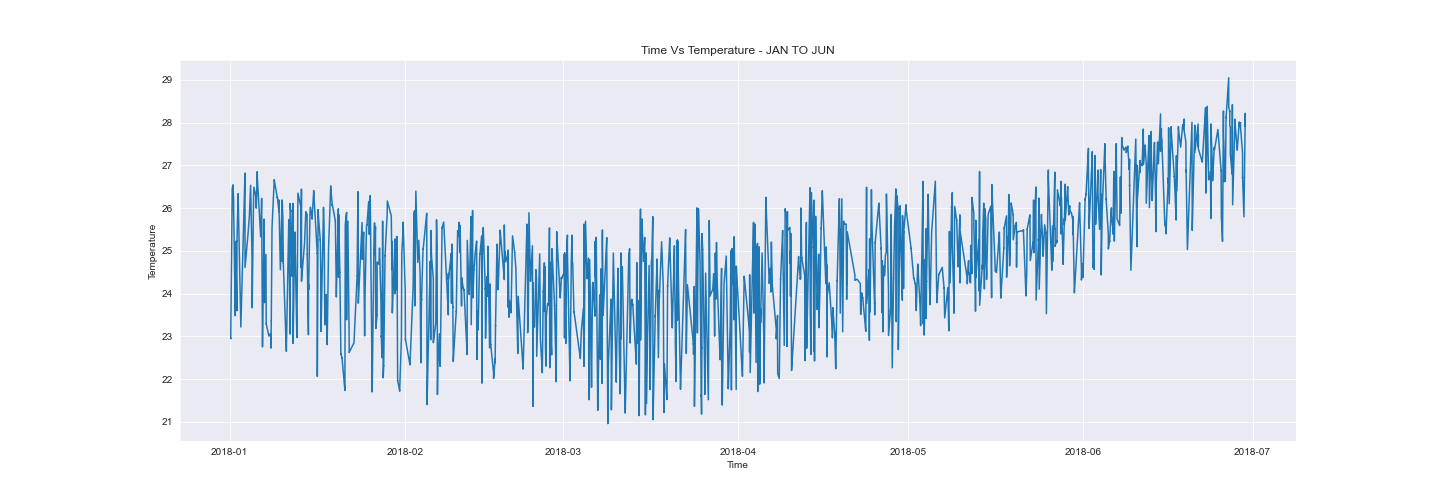
\includegraphics[width=1\textwidth]{JAN_JUN.png} % Include the image placeholder.png
\caption{JANUARY TO JUNE 2018.}
\end{center}
\end{figure}

\begin{figure}[h]
\begin{center}
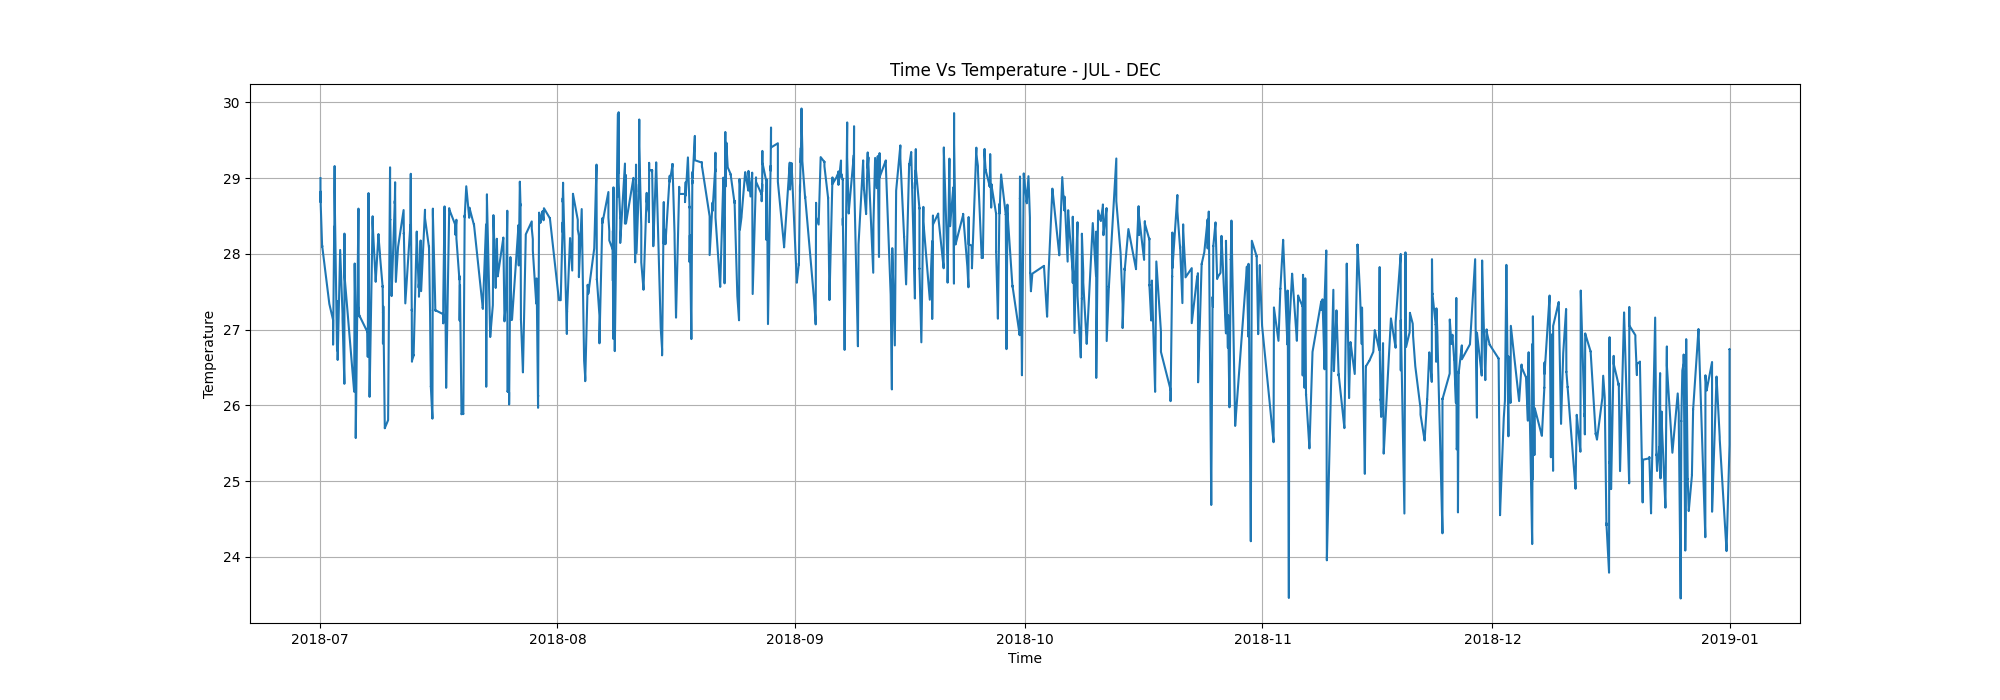
\includegraphics[width=1\textwidth]{JUL_DEC.png} % Include the image placeholder.png
\caption{JULY TO DECEMBER 2018}
\end{center}
\end{figure}

%----------------------------------------------------------------------------------------
%	SECTION 4
%----------------------------------------------------------------------------------------

\section{Results and Conclusion}
The zigzag pattern of the figures above represents the movement of the float. Temperatures start to  drop in August as winter season approaches.

There is a rise in Temperature from March, this represents the end of the winter and the beginning of the spring/summer season

%----------------------------------------------------------------------------------------
%	BIBLIOGRAPHY
%----------------------------------------------------------------------------------------

\section{BIBLIOGRAPHY}
\bibliographystyle{apalike}

\bibliography{sample}
\begin{enumerate}
\item Argo data python library - \url{ https://argopy.readthedocs.io/en/latest/index.html}
\end{enumerate}

%----------------------------------------------------------------------------------------


\end{document}